\Needspace{12\baselineskip}
\section{西安算例的补充结果}
\label{sec:sup:xian}
西安参数见正文表~\ref{tab:xian_initial_fit}，计算使用 $I_0$ 的未取整值。

\subsection{人口缩放}
\label{sec:sup:xian:settings}
人口缩放情景取 $N=N_{\rm eff}$、$S_0=N-I_0$，沿用全市拟合的绝对初值 $I_0$ 与传播参数，其余初始仓室为零，不重新拟合。它同时改变 $N$、$i_0=I_0/N$ 与 $\eta=\theta N$。固定 $\theta=0.002$、取 $N\in\{5\times10^4,10^5,5\times10^5,10^6,5\times10^6,1.3163\times10^7\}$ 的六个人口规模，仅隔离控制的控制时长均约为 $85.07$ 天，$\Delta t$ 和 $J$ 的相对极差分别为 $4.71\times10^{-8}$ 和 $1.17\times10^{-7}$；以 $t-t_1$ 为时间变量时，归一化感染轨迹和隔离比例近似重合。启动时间由 $11.39$ 天增加至 $16.90$ 天，这是固定绝对初值时，初始感染比例 $i_0=I_0/N$ 随 $N$ 增大而减小的结果：初期近似指数增长，$t_1\approx g^{-1}\ln(\theta/i_0)$，其中 $g=\beta c_0(1-q_0)-\gamma$ 为初期增长率。固定绝对阈值 $\eta=100$、把 $N$ 从 $1.3163\times10^7$ 降到 $5\times10^4$ 时，$\theta=\eta/N$ 增大，控制时长由约 $2.25\times10^4$ 天缩短到约 $85$ 天。两组结果都符合
\[
\Delta t=\frac1{c_0\theta}\ln\frac{s^*-\bar s}{s_c-\bar s},
\]
其中对数因子在 $\theta\in[5\times10^{-4},8\times10^{-3}]$ 内仅由 $2.20$ 变到 $2.15$，因此 $\Delta t$ 近似与 $\theta$ 成反比。

固定归一化初值时，以绝对终点 $I=1$ 计的量随人口单调变化。记 $i_{\max}^{0}=I_{\max}^{0}/N$（式\eqref{eq:s1:Imax-no}），固定归一化初值 $s_0,i_0$ 时它不依赖 $N$。
\begin{proposition}
\label{prop:reference-population}
固定 $s_0,i_0,\theta$ 和模型参数，且 $i_0<\theta<i_{\max}^{0}$。在 $N\theta>1$ 的范围内，仅隔离控制的清零时间、计算至该终点的累计新增感染及其占人口的比例均随 $N$ 严格增加。
\end{proposition}
\begin{proof}
归一化轨迹及启动、控制时长与 $N$ 无关。退出后 $i(t)$ 从 $\theta$ 严格下降至零，终点为 $i=1/N$。增大 $N$ 使终点更低，故清零时间严格增加。

记 $s_{\rm end}=S_{\rm end}/N$。归一化的退出后首次积分为
\[
\frac1N=\theta+\frac{\beta_2^0}{\beta_1^0}(s_c-s_{\rm end})
+\frac{\rho_1}{N}\ln\frac{s_{\rm end}}{s_c},
\]
其中 $\rho_1/N$ 与 $\beta_2^0/\beta_1^0$ 均不随 $N$ 改变。于是
\[
\frac{\partial s_{\rm end}}{\partial N}
=-\frac1{N^2(\rho_1/N)(1/s_{\rm end}-1/s_c)}<0.
\]
将式\eqref{eq:s1:cumulative}除以 $N$ 后，只有 $s_{\rm end}$ 含 $N$，因而比例满足
\[
\frac{\partial(\Itcum/N)}{\partial N}
=-\frac{\beta}{\beta+q_0(1-\beta)}\frac{\partial s_{\rm end}}{\partial N}>0,
\]
人数满足
\[
\frac{\partial\Itcum}{\partial N}
=\frac{\Itcum}{N}
-\frac{N\beta}{\beta+q_0(1-\beta)}\frac{\partial s_{\rm end}}{\partial N}>0.\qedhere
\]
\end{proof}
命题不适用于固定绝对阈值或固定绝对 $I_0$ 的比较，后者见上一段。

\FloatBarrier
\subsection{阈值扫描}
\label{sec:sup:xian:threshold-scan}
表~\ref{tab:sup:eta}与图~\ref{fig:xian_eta_sens}给出 11 个阈值比例下仅隔离控制的结果，覆盖设计阈值 $\eta/N=0.002$ 的两侧。阈值从 $0.01N$ 降到 $0.0001N$ 时，$q_{\max}$ 只在 $0.838$ 与 $0.847$ 之间变化，控制时长与成本近似按阈值的反比增加，总累计新增感染则缓慢减少；正文第~\ref{sec:xian:threshold-scale}~节由此解释低阈值的代价。
\begin{table}[htbp]
\centering\small
\setlength{\tabcolsep}{3.5pt}
\renewcommand{\arraystretch}{1.25}
\begin{threeparttable}
\caption{西安参数下不同阈值的仅隔离控制}
\label{tab:sup:eta}
\begin{tabular*}{\linewidth}{@{\extracolsep{\fill}}S[table-format=1.4]S[table-format=1.4]S[table-format=4.2]S[table-format=4.2]S[table-format=3.4]S[table-format=7.0]@{}}
\toprule
{$\eta/N$} & {$q_{\max}$} & {$\Delta t$（d）} & {$t_{\rm end}$（d）} & {$J$（d）} & {\shortstack{总累计新增感染\\（人）}}\\
\midrule
0.0001 & 0.8470 & 1710.66 & 2209.55 & 826.4066 & 2155649\\
0.0002 & 0.8469 & 855.09 & 1243.15 & 412.9141 & 2182123\\
0.0005 & 0.8466 & 341.75 & 620.77 & 164.8184 & 2234666\\
0.0010 & 0.8462 & 170.63 & 389.32 & 82.1192 & 2293939\\
0.0015 & 0.8458 & 113.59 & 304.01 & 54.5524 & 2339486\\
0.0020 & 0.8454 & 85.07 & 258.10 & 40.7686 & 2377943\\
0.0030 & 0.8445 & 56.55 & 208.39 & 26.9842 & 2442608\\
0.0040 & 0.8436 & 42.29 & 181.18 & 20.0913 & 2497306\\
0.0050 & 0.8428 & 33.73 & 163.65 & 15.9550 & 2545663\\
0.0075 & 0.8405 & 22.32 & 138.10 & 10.4383 & 2649240\\
0.0100 & 0.8382 & 16.61 & 123.89 & 7.6781 & 2737382\\
\bottomrule
\end{tabular*}
\begin{tablenotes}[flushleft]\footnotesize
\item 注：$q_{\max}=q_c(t_1)$；$\eta/N$ 为比例，$0.002$ 即 $0.2\%$；总累计新增感染计算至清零时间。
\end{tablenotes}
\end{threeparttable}
\end{table}

\begin{figure}[htbp]
    \centering
    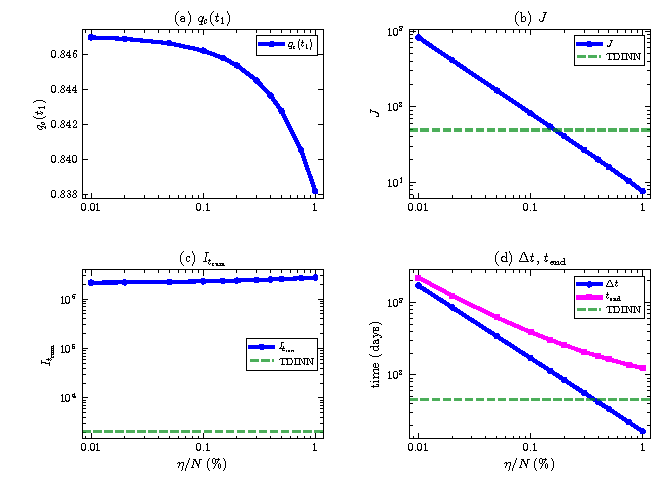
\includegraphics[width=0.7\textwidth]{new4o/xian_eta_sensitivity.pdf}
    \caption{西安参数下仅隔离控制的指标随 $\eta/N$ 的变化：(a) 启动时的隔离比例；(b) 成本 $J$；(c) 累计新增感染；(d) 控制时长与清零时间。水平虚线为 TDINN 参照值，其中 TDINN 的 $J$ 用同一二次强度被积函数与默认权重在 $[0,t_{\rm end}^{\rm T}]$ 上积分；(d) 中 TDINN 的控制时长与清零时间同为 $45.29$ d。}
    \label{fig:xian_eta_sens}
\end{figure}

图~\ref{fig:xian_heatmaps}把扫描推广到 $(\eta,c_0)$ 平面。在图示的 $c_0$ 范围内，控制时长、清零时间与成本的等值线接近竖直，主要由阈值决定；正文第~\ref{sec:xian:threshold-scale}~节在 TDINN 峰值处的控制时长即取自子图 (a)。
\begin{figure}[htbp]
    \centering
    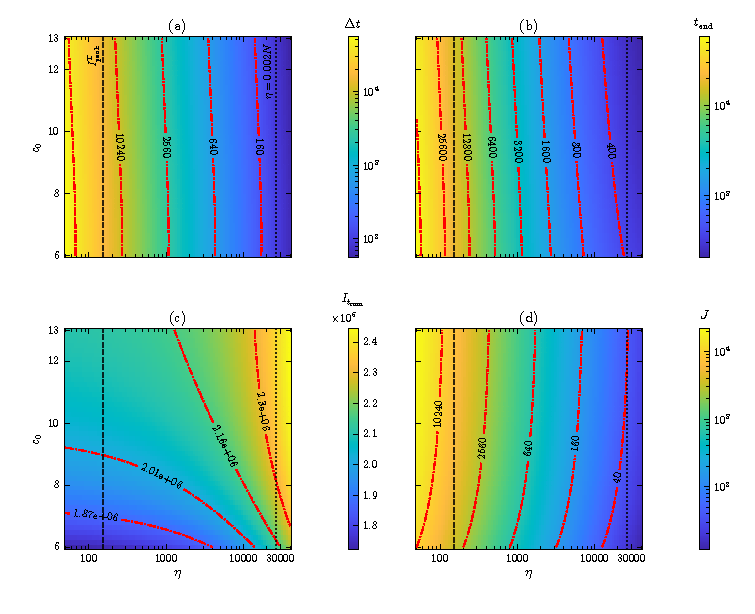
\includegraphics[width=0.8\textwidth]{figures/new4t/S8.pdf}
    \caption{西安参数下仅隔离控制在 $(\eta,c_0)$ 平面上的指标：(a) 控制时长；(b) 清零时间；(c) 累计新增感染；(d) 成本 $J$。两条竖直参照线分别为 TDINN 的非隔离感染者峰值 $\eta=152.55$ 与设计阈值 $\eta=26326$；红色点划线为等值线，黑色数字为等值。}
    \label{fig:xian_heatmaps}
\end{figure}

\subsection{设计阈值的量级}
\label{sec:sup:threshold-scale}
正文西安算例取 $N=13{,}163{,}000$\cite{XianStat2021}、$\eta=0.002N=26{,}326$。这一阈值来自下面的量级估计，它与第~\ref{sec:sup:medical-link}~节的充分条件是两种不同的依据。

陈胤孜等\cite{Chen2021ICUForecast}基于既往资料预测，2021 年全国每10万人综合 ICU 床位约为 $4.37$ 张；这一数值为全国预测量，而非西安同期可用容量的实测值。Angulo 等\cite[补充材料 S4.1]{Angulo2021}对早期 COVID-19 采用需要重症监护的感染者比例名义值 $0.60\times0.15\times0.28=0.0252$。将前者作为人均容量参考、不扣除既有占用，并将后者移作参考系数 $\rho_{\mathrm{ICU}}$，按比例情景
\[
\eta=\frac{C}{\rho_{\mathrm{ICU}}},\qquad
\theta=\frac{C/N}{\rho_{\mathrm{ICU}}}
\]
得到
\[
\theta=\frac{4.37/10^5}{0.0252}\approx1.73\times10^{-3},
\qquad \eta\approx2.28\times10^4.
\]
正文在这一量级附近取 $\theta=0.002$ 作为设计情景。按相同的参考系数反算，它对应每10万人 $5.04$ 张、全市约 $663$ 张的名义容量。

这一比例移植只给出阈值的量级，不是当地医疗容量的临床校准。以确诊病例或全部感染者为分母的 ICU 入院风险可能不同\cite{Pung2023Undetected}；参考系数 $\rho_{\mathrm{ICU}}$ 也没有依据共同的需求函数和初始负担估计，不等同于第~\ref{sec:sup:medical-link}~节中的 $pL\beta c_0S_0/N$。

\FloatBarrier
